\documentclass[letterpaper,12pt]{article}
\usepackage[utf8]{inputenc}
\usepackage{fullpage}
\usepackage{courier}
\usepackage[margin=0.75in]{geometry}
\usepackage{listings}
\usepackage{color}
\usepackage{graphicx}
\usepackage[width=5in]{caption}
\usepackage{hyphenat}
\usepackage[section]{placeins}
\usepackage{cmll}
\usepackage{float}
\usepackage{hyperref}

% Format a sectionless paragraph
\newcommand*\unparagraph{
	\par
	\nopagebreak
	\vskip3.25ex plus1ex minus.2ex
	\noindent
}

% define extra colors
\definecolor{dkgreen}{rgb}{0,0.6,0}
\definecolor{purple}{RGB}{159,0,197}

% define the code listing format
\lstset{
	language=Python,
	basicstyle=\footnotesize\ttfamily,
	backgroundcolor=\color{white},
	showspaces=false,
	showstringspaces=false,
	frame=none,
	tabsize=3,
	keywordstyle=\color{purple},
	commentstyle=\color{dkgreen},
	stringstyle=\color{blue},
	escapeinside={\%*}{*)}
}

% define the title/header
\title{\Large CS 1428 Honors\\Lab 11}
\author{Jared Wallace}
\date{}

\begin{document}

\maketitle

\vspace{30mm}

\section*{Overview}
Today we will be entering the wild world of Python. Python is very different from
C++. One of the main differences is that Python is not compiled, but rather interpreted. Another
big difference is that Python uses whitespace instead of curly braces.

A brief listing of pros and cons of Python are below.
\begin{itemize}
    \item The interpreter allows instant testing
    \item Focus on problem solving, not details and syntax (for the most part)
    \item Code is very elegant looking
    \item Python is always slower than the equivalent C or C++ code
    \item It can be unclear why your program doesn't work sometimes, due to the nature of non static typing
\end{itemize}

Here's an example Python program that prints "Hello World"
\begin{lstlisting}
    #!/usr/bin/python
    print "Hello World"
\end{lstlisting}
That's all the code you need.

Python does not have "arrays" per se, but it does have \textbf{lists}. A list is simply a collection of things.
You can even have a list of lists if you really want. Getting the values out of a list is super easy as well.
For example, I'll create a list with the numbers 1-9 and print them out. To open the interpreter directly, just type
"python" into the terminal.
\begin{lstlisting}
>>>myList = [1,2,3,4,5,6,7,8,9]
>>>print myList
[1,2,3,4,5,6,7,8,9]
\end{lstlisting}

Well, what if we don't want the entire list at once? Python offers a very easy method for looping, called
for each. Remember, whitespace (spaces, tabs) matters in Python!
\begin{lstlisting}
>>>for element in myList:
... print element
...
1
2
3
4
5
6
7
8
9
\end{lstlisting}

Python also offers many different ways to manipulate the list, like reverse() and sort().

\section*{Problems}
\begin{enumerate}
    \item (30 pts) Write a program to add all the natural numbers below 1000 that are multiples of 3 or 5.
    \item (70 pts) Write a program to add all the even numbers in the fibonacci sequence below 4,000,000
\end{enumerate}

\section*{Bonus}
Create a webpage today (don't worry, I'll give you the HTML part)
that aggregates RSS feeds and displays them upon page load. We will be using an API, or Application
Program Interface, located at the following address: \url{https://wiki.python.org/moin/RssLibraries}.

Note: You will need to make your file world readable and executable by executing the following line in the terminal.
\begin{lstlisting}
chmod 755 index.py
\end{lstlisting}

This bonus is worth 20 points on your lowest lab grade.

\section*{Deliverables}
Hard copies of the source code you wrote (multiple.py and fibonacci.py). Soft copy (upload to homework upload) of
your source code. You may, at your discretion, use Git for version control -- it is not required.

% Comic at the bottom
\begin{figure}[ht!]
\centering
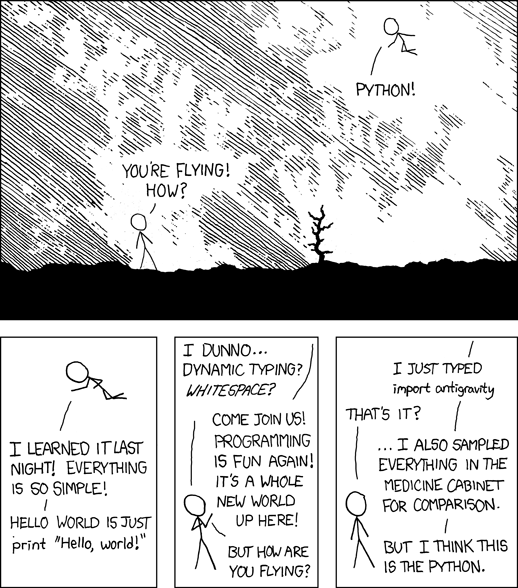
\includegraphics[width=6in]{python.png}
\caption*{"I wrote 20 short programs in Python yesterday.  It was wonderful.  Perl, I'm leaving you."}
\end{figure}
\end{document}
